\PassOptionsToPackage{table}{xcolor}
\documentclass{beamer}\usepackage[]{graphicx}\usepackage[]{color}
%% maxwidth is the original width if it is less than linewidth
%% otherwise use linewidth (to make sure the graphics do not exceed the margin)
\makeatletter
\def\maxwidth{ %
  \ifdim\Gin@nat@width>\linewidth
    \linewidth
  \else
    \Gin@nat@width
  \fi
}
\makeatother

\definecolor{fgcolor}{rgb}{0.345, 0.345, 0.345}
\newcommand{\hlnum}[1]{\textcolor[rgb]{0.686,0.059,0.569}{#1}}%
\newcommand{\hlstr}[1]{\textcolor[rgb]{0.192,0.494,0.8}{#1}}%
\newcommand{\hlcom}[1]{\textcolor[rgb]{0.678,0.584,0.686}{\textit{#1}}}%
\newcommand{\hlopt}[1]{\textcolor[rgb]{0,0,0}{#1}}%
\newcommand{\hlstd}[1]{\textcolor[rgb]{0.345,0.345,0.345}{#1}}%
\newcommand{\hlkwa}[1]{\textcolor[rgb]{0.161,0.373,0.58}{\textbf{#1}}}%
\newcommand{\hlkwb}[1]{\textcolor[rgb]{0.69,0.353,0.396}{#1}}%
\newcommand{\hlkwc}[1]{\textcolor[rgb]{0.333,0.667,0.333}{#1}}%
\newcommand{\hlkwd}[1]{\textcolor[rgb]{0.737,0.353,0.396}{\textbf{#1}}}%

\usepackage{framed}
\makeatletter
\newenvironment{kframe}{%
 \def\at@end@of@kframe{}%
 \ifinner\ifhmode%
  \def\at@end@of@kframe{\end{minipage}}%
  \begin{minipage}{\columnwidth}%
 \fi\fi%
 \def\FrameCommand##1{\hskip\@totalleftmargin \hskip-\fboxsep
 \colorbox{shadecolor}{##1}\hskip-\fboxsep
     % There is no \\@totalrightmargin, so:
     \hskip-\linewidth \hskip-\@totalleftmargin \hskip\columnwidth}%
 \MakeFramed {\advance\hsize-\width
   \@totalleftmargin\z@ \linewidth\hsize
   \@setminipage}}%
 {\par\unskip\endMakeFramed%
 \at@end@of@kframe}
\makeatother

\definecolor{shadecolor}{rgb}{.97, .97, .97}
\definecolor{messagecolor}{rgb}{0, 0, 0}
\definecolor{warningcolor}{rgb}{1, 0, 1}
\definecolor{errorcolor}{rgb}{1, 0, 0}
\newenvironment{knitrout}{}{} % an empty environment to be redefined in TeX

\usepackage{alltt}

\mode<presentation>
{
  \usetheme{Warsaw}
  
}

\beamertemplatenavigationsymbolsempty 

\usepackage[]{inputenc}
\usepackage[english]{babel}
\usepackage{amsthm}
\usepackage{graphicx}
\usepackage{epstopdf}
\usepackage{grffile}
\usepackage{hyperref}
\usepackage{beamerthemesplit}
\definecolor{links}{HTML}{2A1B81}
\hypersetup{colorlinks,linkcolor=,urlcolor=links}
%\setsansfont[Ligatures={Common,TeX}]{TeX Gyre Heros}

{\renewcommand{\arraystretch}{1.1}

\AtBeginSection[]
{
  \begin{frame}
    \frametitle{Outline}
    \tableofcontents[currentsection]
  \end{frame}
}

\newcommand*\oldmacro{}%
\let\oldmacro\insertshorttitle%
\renewcommand*\insertshorttitle{%
   \oldmacro\hfill%
   \insertframenumber\,/\,\inserttotalframenumber}

\setbeamertemplate{headline}{}
\setbeamertemplate{itemize items}[circle]
\title[SHM model based on synonymous mutations]{Models of somatic hypermutation targeting and substitution based on synonymous mutations
    from high-throughput immunoglobulin sequencing data}

    \author [Andrey Bzikadze]{Andrey Bzikadze}
%\institute{Saint Petersburg State University, Russia \\
%           Faculty of Mathematics and Mechanics \\
%           Department of Statistical Modelling}
\date {
February 12, 2016
}

\usepackage[absolute,overlay]{textpos}
\setlength{\TPHorizModule}{1cm} % Horizontale Einheit
\setlength{\TPVertModule}{1cm} % Vertikale Einheit
\addtobeamertemplate{title page}{
}{}
\IfFileExists{upquote.sty}{\usepackage{upquote}}{}

\begin{document}
\begin{frame}
  \titlepage
\end{frame}

\section{Introduction}

\begin{frame}{Introduction: \texttt{V(D)J-recombination}}
  Immunoglobulin heavy chain locus:
  \begin{figure}[h]
    \center\includegraphics[width=300pt]{Pictures/vdj1.pdf}
 \end{figure}
\end{frame}

\begin{frame}{Introduction: \texttt{V(D)J-recombination}}
  Segment of each type is selected: 
  \begin{figure}[h]
    \center\includegraphics[width=300pt]{Pictures/vdj2_select_genes.pdf}
 \end{figure}
\end{frame}

\begin{frame}{Introduction: \texttt{V(D)J-recombination}}
  3 types of biochemical events: \textit{palindrome}, \textit{cleavage}, \textit{non-genomic insertion}. 
  \begin{figure}[h]
    \center\includegraphics[width=300pt]{Pictures/vdj3_DJ_aligned_new.pdf}
 \end{figure}
\end{frame}

\begin{frame}{Introduction: \texttt{V(D)J-recombination}}
  Further optimization of antibody affinity is achieved through extensive mutations referred as \textit{somatic hypermutations}:
  \begin{figure}[h]
    \center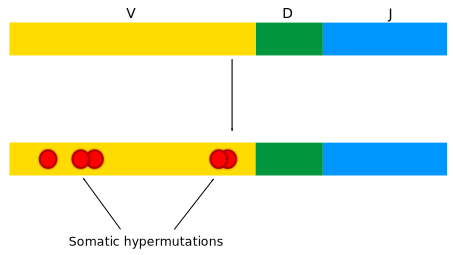
\includegraphics[width=300pt]{Pictures/somatic_mutations.pdf}
 \end{figure}
\end{frame}

\begin{frame}{Introduction: \texttt{V(D)J-recombination}}
    Because we do not know the deterministic nature of the \texttt{V(D)J-recombination} and \texttt{hypermutations}, it is reasonable
  to consider it as a {\color{blue} random} (stochastic) process.

  \bigskip
  Hence the analysis of somatic recombination and hypermutations can be done in statistical and simulation terms. 
\end{frame}

\begin{frame}{Introduction: ``\texttt{hot}'' and ``\texttt{cold}'' spots}
  \begin{figure}[h]
    \center\includegraphics[width=280pt]{Pictures/Hot_and_cold_spots.pdf}
 \end{figure}
\end{frame}

\begin{frame}{Introduction: surrounding basis}
    \href{http://www.sciencedirect.com/science/article/pii/S0161589011001192}{
    Reuma Magori Cohen, Steven H. Kleinstein, Yoram Louzoun, Somatic hypermutation targeting is influenced by location within the immunoglobulin V region, Molecular Immunology, 2011.}
  \begin{figure}[h]
    \center\includegraphics[width=250pt]{Pictures/three_surround.pdf}
 \end{figure}
\end{frame}

\section{SHM models based on synonymous mutations}
\begin{frame}
    \frametitle{SHM models based on 5-mers:}
    \href{http://journal.frontiersin.org/article/10.3389/fimmu.2013.00358/abstract}{Gur Yaari \textit{et. al.},
        Models of somatic hypermutation targeting and substitution based on synonymous mutations
        from high-throughput immunoglobulin sequencing data --- Front. Immunol., 2013}.
    \pause
    \bigskip
    \begin{columns}[c]
        \begin{column}{0.4\textwidth}
            \ \, \quad A \textbf{targeting}
            model.
            \begin{table}[]
                \centering
                \begin{tabular}{c|c}
                5-mer & Mutability \\ \hline
                    \ldots & \ldots \\
                    GC{\color{red}C}TC & 0.12       \\
                    GC{\color{red}G}AC & 0.16       \\
                    AC{\color{red}A}CT & 0.48       \\
                    AG{\color{red}C}TA & 3.17       \\
                    \ldots & \ldots
                \end{tabular}
            \end{table}
        \end{column}
        \pause
        \begin{column}{0.6\textwidth}
            \qquad A nucleotide \textbf{substitution} model.
            \begin{table}[]
                \centering
                \begin{tabular}{c|c|c|c|c}
                    5-mer & \multicolumn{1}{c|}{A} & \multicolumn{1}{c|}{C} & \multicolumn{1}{c|}{G} & T   \\ \hline
                    \ldots & \ldots & \ldots & \ldots  & \ldots \\
                    AC{\color{red}A}AC   & 0                      & .24                    & .48                    & .29 \\
                    GG{\color{red}C}GT   & .22                    & 0                      & .12                    & .65 \\
                    CC{\color{red}G}TC   & .35                    & .52                    & 0                      & .13 \\
                    TC{\color{red}T}AC   & .31                    & .54                    & .14                    & 0   \\
                    \ldots & \ldots & \ldots & \ldots  & \ldots
                \end{tabular}
            \end{table}
        \end{column}
    \end{columns}
\end{frame}

\begin{frame}
    \frametitle{Bias of the selection}
    The standard solution: use \textbf{non-productively} rearranged Ig genes.
    (for example, \href{http://www.pnas.org/content/109/40/16161.full}{%Statistical inference of the generation probability of \texttt{T}-cell receptors from sequence repertoires (
    Anand Murugana, Thierry Morab, Aleksandra M. Walczak and Curtis G. Callan --- 2012}).

    \bigskip
    \pause
    {\color{blue} Authors point}: ``non-productively rearranged Ig genes may still be influenced by selection''.\\

    \bigskip
    {\color{blue} Authors solution}: ``developed a new methodology for constructing models from \textbf{synonymous}
mutations only, thus avoiding the need to limit analysis
to non-productive Ig sequences''.
\end{frame}


\section{Datasets and pre-processing}
\begin{frame}
    \frametitle{Used datasets}
    { \footnotesize
    \begin{table}[]
    \centering
    \begin{tabular}{ccccccc}
    \hline
    \multicolumn{1}{|c|}{\bf Subj.}   & \multicolumn{1}{c|}{\bf Tech.} & \multicolumn{1}{c|}{\bf Raw }  & \multicolumn{1}{c|}{\bf Processed} \\ \hline
    \multicolumn{1}{|c|}{1}           & \multicolumn{1}{c|}{MiSeq}     & \multicolumn{1}{c|}{3,641,633} & \multicolumn{1}{c|}{79,777   }     \\
    \multicolumn{1}{|c|}{2}           & \multicolumn{1}{c|}{MiSeq}     & \multicolumn{1}{c|}{3,714,152} & \multicolumn{1}{c|}{106,006  }     \\
    \multicolumn{1}{|c|}{3}           & \multicolumn{1}{c|}{MiSeq}     & \multicolumn{1}{c|}{10,917,517}& \multicolumn{1}{c|}{231,387  }     \\
    \multicolumn{1}{|c|}{4}           & \multicolumn{1}{c|}{MiSeq}     & \multicolumn{1}{c|}{7,691,509} & \multicolumn{1}{c|}{99,519   }     \\ \cline{1-4}
    \multicolumn{1}{|c|}{5}           & \multicolumn{1}{c|}{MiSeq}     & \multicolumn{1}{c|}{3,851,658} & \multicolumn{1}{c|}{55,606   }     \\
    \multicolumn{1}{|c|}{5}           & \multicolumn{1}{c|}{MiSeq}     & \multicolumn{1}{c|}{3,946,514} & \multicolumn{1}{c|}{59,611   }     \\
    \multicolumn{1}{|c|}{5}           & \multicolumn{1}{c|}{MiSeq}     & \multicolumn{1}{c|}{4,543,353} & \multicolumn{1}{c|}{48,971   }     \\
    \multicolumn{1}{|c|}{5}           & \multicolumn{1}{c|}{MiSeq}     & \multicolumn{1}{c|}{3,121,884} & \multicolumn{1}{c|}{52,844   }     \\ \cline{1-4}
    \multicolumn{1}{|c|}{5}           & \multicolumn{1}{c|}{454}       & \multicolumn{1}{c|}{117,188}   & \multicolumn{1}{c|}{71,043   }     \\
    \multicolumn{1}{|c|}{6}           & \multicolumn{1}{c|}{454}       & \multicolumn{1}{c|}{178,584}   & \multicolumn{1}{c|}{92,055   }     \\
    \multicolumn{1}{|c|}{7}           & \multicolumn{1}{c|}{454}       & \multicolumn{1}{c|}{398,517}   & \multicolumn{1}{c|}{248,363  }     \\ \hline
    \multicolumn{1}{|c|}{Total}       & \multicolumn{1}{c|}{---}       & \multicolumn{1}{c|}{42,122,509}& \multicolumn{1}{c|}{1,145,182}     \\ \cline{1-4}
    \end{tabular}
    \end{table}
    }

{\color{blue} Each sample was uniquely barcoded.}
\end{frame}

\begin{frame}
    \frametitle{Pre-processing (\texttt{pRESTO}): quality control}
    \begin{itemize}
        \item Removal of low-quality reads (mean Phred quality sc. $<20$).
        \item For the MiSeq data, sets of sequences with identical molecular
IDs were
identified. Sets were collapsed into one consensus sequence
per set.
        \pause
        \item Removal of sequences that do not appear in a single sample
            at least \textbf{twice}.
    \end{itemize}
\end{frame}

\begin{frame}{Pre-processing (\texttt{pRESTO})}
    \begin{itemize}
        \item Alignment --- IMGT/HighV-QUEST.
        \item
            Non-mutated sequences: choice of V gene if $> 0.1\%$ of the
            sequences; choice of V gene alleles if $ > 10\%$ of
            the assignments to this V gene.
        \item Mutated sequences: closest V segment due Hamming distance.
        %\item Removal of non-fuctional seqs (stop codon or frame shift).
        %\item Removal of seqs with $>30$ mutations.
        %\item Removal of mutations in codon if more than one mutation occured.
    \end{itemize}
\end{frame}

\begin{frame}{Pre-processing (\texttt{pRESTO}): clonally related sequences}

    {\color{blue} Clones --- the sequences related by a common ancestor.} 

    Identification of clonally related sequences:
    \begin{enumerate}
        \item Clusterization based on V, J alignment and junction.
        \item Clones, if junctions differ by $\le 3$ mutations.
    \end{enumerate}

    \bigskip
    \begin{quote}
        ``The threshold of three was determined after manual inspection
        of the mutation patterns in resulting clones identified through
        building lineage trees.''
    \end{quote}
\end{frame}

\section{Substitution model}

\begin{frame}
    \frametitle{Substitution model}
    Consider only 5-mers where \textbf{any} mutation at central position is synonymous.
    { \footnotesize
    \begin{table}[]
    \centering
    \begin{tabular}{ccccccc}
    \hline
    \multicolumn{1}{|c|}{\bf Subj.}   & \multicolumn{1}{c|}{\bf Tech.} & \multicolumn{1}{c|}{\bf Processed} & \multicolumn{1}{c|}{\# \bf Subst. mut.}  \\ \hline
    \multicolumn{1}{|c|}{1}           & \multicolumn{1}{c|}{MiSeq}     & \multicolumn{1}{c|}{79,777   }     & \multicolumn{1}{c|}{25,307 }           \\
    \multicolumn{1}{|c|}{2}           & \multicolumn{1}{c|}{MiSeq}     & \multicolumn{1}{c|}{106,006  }     & \multicolumn{1}{c|}{57,215 }           \\
    \multicolumn{1}{|c|}{3}           & \multicolumn{1}{c|}{MiSeq}     & \multicolumn{1}{c|}{231,387  }     & \multicolumn{1}{c|}{108,591}           \\
    \multicolumn{1}{|c|}{4}           & \multicolumn{1}{c|}{MiSeq}     & \multicolumn{1}{c|}{99,519   }     & \multicolumn{1}{c|}{68,051 }           \\ \cline{1-4}
    \multicolumn{1}{|c|}{5}           & \multicolumn{1}{c|}{MiSeq}     & \multicolumn{1}{c|}{55,606   }     & \multicolumn{1}{c|}{23,939 }           \\
    \multicolumn{1}{|c|}{5}           & \multicolumn{1}{c|}{MiSeq}     & \multicolumn{1}{c|}{59,611   }     & \multicolumn{1}{c|}{24,971 }           \\
    \multicolumn{1}{|c|}{5}           & \multicolumn{1}{c|}{MiSeq}     & \multicolumn{1}{c|}{48,971   }     & \multicolumn{1}{c|}{20,865 }           \\
    \multicolumn{1}{|c|}{5}           & \multicolumn{1}{c|}{MiSeq}     & \multicolumn{1}{c|}{52,844   }     & \multicolumn{1}{c|}{23,243 }           \\ \cline{1-4}
    \multicolumn{1}{|c|}{5}           & \multicolumn{1}{c|}{454}       & \multicolumn{1}{c|}{71,043   }     & \multicolumn{1}{c|}{8,209  }           \\
    \multicolumn{1}{|c|}{6}           & \multicolumn{1}{c|}{454}       & \multicolumn{1}{c|}{92,055   }     & \multicolumn{1}{c|}{23,260 }           \\
    \multicolumn{1}{|c|}{7}           & \multicolumn{1}{c|}{454}       & \multicolumn{1}{c|}{248,363  }     & \multicolumn{1}{c|}{24,771 }           \\ \hline
    \multicolumn{1}{|c|}{Total}       & \multicolumn{1}{c|}{---}       & \multicolumn{1}{c|}{1,145,182}     & \multicolumn{1}{c|}{408,422}           \\ \cline{1-4}
    \end{tabular}
    \end{table}
    }
\end{frame}

\begin{frame}
    \frametitle{Substitution model: definition}
    For each $5$-mer $M$ let central base mutate to $B \in \{\mathrm A, \mathrm  C,  \mathrm G, \mathrm T\}$.
    The model is the set of probabilities for mutation of $M$ to $B$.
    Estimations are frequencies.

\end{frame}

\begin{frame}
    \frametitle{Substitution model: inferred estimations}
    \begin{itemize}
        \item Not all 5-mers appear in datasets.
        \item Some 5-mers can never appear: not all substitutions are synonymous.
   \end{itemize}
  \begin{figure}[h]
      \center\includegraphics[width=200pt]{Pictures/synonymous_mutations.pdf}
 \end{figure}
   \pause
   \bigskip
       { \color{blue} Substitutions for 717 (of 1024) 5-mers were not estimated! }
\end{frame}

\begin{frame}
    \frametitle{Substitution model: inferred estimations}
    To estimate, for example, $\mathbb P(\mathrm{CA{\color{red} L}AG} \to \mathrm{CA{\color{red}M}AG})$:%, where $\mathrm{L, M} \in \{\mathrm{A, C, G, T}\}$:
    \begin{itemize}
        \item ``inner 3-mer'':
            \hfill    ${\mathbb P(\mathrm{*\,A{\color{red}L}A\,*} \to \, \mathrm{*A\,{\color{red}M\,}A*})}$;
        \item 2 upstream nucleotides:
            \hfill ${\mathbb P(\mathrm{CA{\color{red}L}**} \to \mathrm{CA{\color{red}M}**})}$;
        \item 2 downstream nucleotides:
            \hfill    ${\mathbb P(\mathrm{**{\color{red}L}AG} \to \mathrm{**{\color{red}M}AG})}$;
        \item ``hot-spot'' method:
                \begin{gather*}
                    \begin{cases}
                        \mathbb P(\mathrm{CA{\color{red}L}**} \to \mathrm{CA{\color{red}M}**}), & \mathrm{L, M} \in \{\mathrm{A, C}\}; \\
                        \mathbb P(\mathrm{**{\color{red}L}AG} \to \mathrm{**{\color{red}M}AG}), & \mathrm{L, M} \in \{\mathrm{G, T}\}. 
                     \end{cases}
                \end{gather*}
    \end{itemize}
    \begin{table}[]
    \centering
    \caption{Corr. between true estimations and inferred for synonymous mutations.}
    \begin{tabular}{ccccc}
    \hline
    Correlation & Inner & Upstream & Downstream & Hot spots \\ \hline
    Pearson     & .4    & .37      & .15        & .04       \\
    Spearman    & .2    & .24      & .23        & .09      
    \end{tabular}
    \end{table}
\end{frame}

\begin{frame}
  \frametitle{Substitutions are affected by adjacent nucleotides}
  \begin{figure}[h]
    \center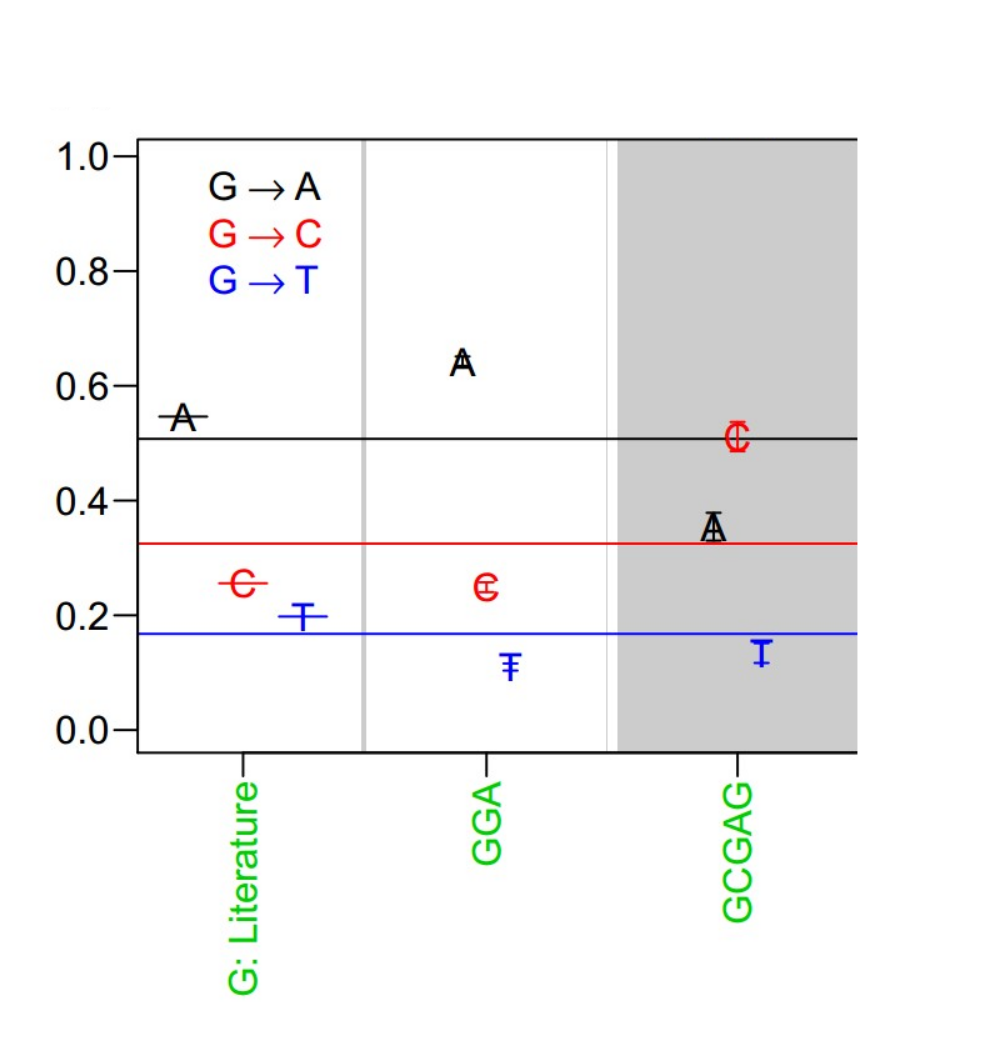
\includegraphics[width=250pt]{Pictures/substitution_adj_nucl.jpg}
 \end{figure}
  \begin{figure}[h]
    \center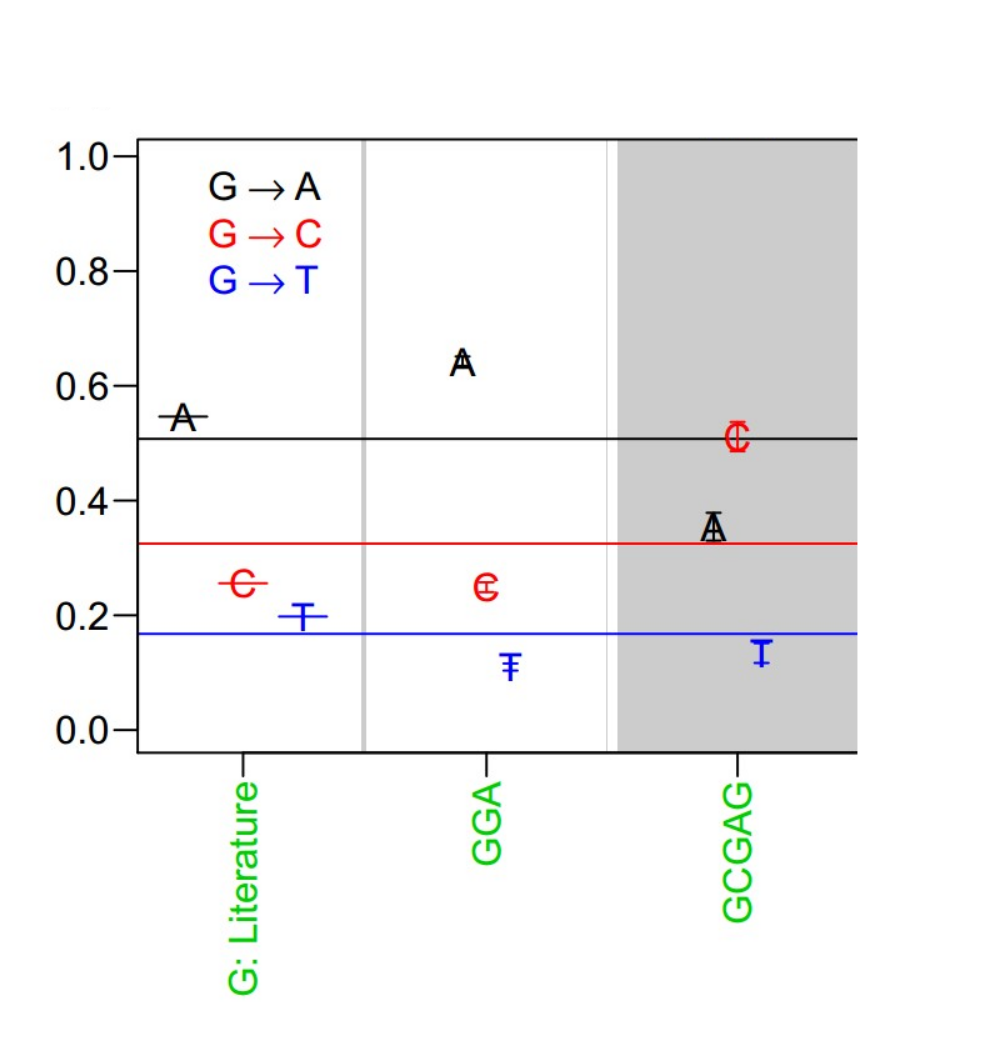
\includegraphics[width=145pt]{Pictures/substitution_adj_nucl.png}
 \end{figure}
\end{frame}

\begin{frame}{Substitution model: comments}
    \textbf{Consistency on different datasets}: in my opinion, the arguments are not convincing
    \begin{itemize}
        \item Bootstrap 95\% CIs often do not overlap.
        \item Correlation between mutations estimated on some of the datasets (esp. 454) is quite low.
    \end{itemize}
    \textbf{Statistical research}: absence of information about
    \begin{itemize}
        \item Significance of the results.
        \item Hypothesis testing about non uniformity of the 5-mer mutations distributions.
        \item Hypothesis testing about non identical distribution of the 5-mer mutations distributions.
    \end{itemize}
\end{frame}
\section{Mutability model}
\begin{frame}
    \frametitle{Mutability model}

    {\color{blue} Only mutations that are synonymous were considered.}
    { \footnotesize
    \begin{table}[]
    \centering
    \begin{tabular}{ccccccc}
    \hline
    \multicolumn{1}{|c|}{\bf Subj.}   & \multicolumn{1}{c|}{\bf Tech.} & \multicolumn{1}{c|}{\bf Processed} & \multicolumn{1}{c|}{\# \bf Targ. mut.}  \\ \hline
    \multicolumn{1}{|c|}{1}           & \multicolumn{1}{c|}{MiSeq}     & \multicolumn{1}{c|}{79,777   }     & \multicolumn{1}{c|}{53,840}           \\
    \multicolumn{1}{|c|}{2}           & \multicolumn{1}{c|}{MiSeq}     & \multicolumn{1}{c|}{106,006  }     & \multicolumn{1}{c|}{106,265}           \\
    \multicolumn{1}{|c|}{3}           & \multicolumn{1}{c|}{MiSeq}     & \multicolumn{1}{c|}{231,387  }     & \multicolumn{1}{c|}{208,338}           \\
    \multicolumn{1}{|c|}{4}           & \multicolumn{1}{c|}{MiSeq}     & \multicolumn{1}{c|}{99,519   }     & \multicolumn{1}{c|}{132,795}           \\ \cline{1-4}
    \multicolumn{1}{|c|}{5}           & \multicolumn{1}{c|}{MiSeq}     & \multicolumn{1}{c|}{55,606   }     & \multicolumn{1}{c|}{48,558}           \\
    \multicolumn{1}{|c|}{5}           & \multicolumn{1}{c|}{MiSeq}     & \multicolumn{1}{c|}{59,611   }     & \multicolumn{1}{c|}{50,117}           \\
    \multicolumn{1}{|c|}{5}           & \multicolumn{1}{c|}{MiSeq}     & \multicolumn{1}{c|}{48,971   }     & \multicolumn{1}{c|}{42,737}           \\
    \multicolumn{1}{|c|}{5}           & \multicolumn{1}{c|}{MiSeq}     & \multicolumn{1}{c|}{52,844   }     & \multicolumn{1}{c|}{47,049}           \\ \cline{1-4}
    \multicolumn{1}{|c|}{5}           & \multicolumn{1}{c|}{454}       & \multicolumn{1}{c|}{71,043   }     & \multicolumn{1}{c|}{48,838}           \\
    \multicolumn{1}{|c|}{6}           & \multicolumn{1}{c|}{454}       & \multicolumn{1}{c|}{92,055   }     & \multicolumn{1}{c|}{50,899}           \\
    \multicolumn{1}{|c|}{7}           & \multicolumn{1}{c|}{454}       & \multicolumn{1}{c|}{248,363  }     & \multicolumn{1}{c|}{17,424}           \\ \hline
    \multicolumn{1}{|c|}{Total}       & \multicolumn{1}{c|}{---}       & \multicolumn{1}{c|}{1,145,182}     & \multicolumn{1}{c|}{806,860}           \\ \cline{1-4}
    \end{tabular}
    \end{table}
    }
\end{frame}

\begin{frame}
    \frametitle{Mutability model: definition}
    \begin{quote}
        ``The mutability of a motif is defined here as the (non-normalized)
        probability of the central base in the motif being targeted for SHM
        relative to all other motifs.''
    \end{quote}
    2 steps:
    \begin{itemize}
        \item  Calculating the \textbf{background frequency} of the
different 5-mers based on the germline (unmutated) version of the
sequence.
        \item  Creating a table of the 5-mers that were mutated
in the sequence.
    \end{itemize}
\end{frame}
\begin{frame}
    \frametitle{Mutability model: definition}
    For each string $S$ let denote $\mathrm {GL}$ --- germline string for string $S$.
    Then for each 5-mer $M$ background frequency is
    \begin{gather*}
        B^S_M = \sum_{i=1}^{\mathrm {Len}(S)} \sum_{b \in ACGT} \mathrm{PrSubst}(M, b) \mathrm{IsSynonymous}(\mathrm{GL}[i], b| M).
    \end{gather*}
    
    \begin{gather*}
        C^S_M = \sum_{i=1}^{\mathrm {Len}(S)} \mathrm{IsSynonymous}(\mathrm{GL}[i], \mathrm{OS}[i]| M).
    \end{gather*}
\end{frame}

\begin{frame}
    \frametitle{Mutability model: definition}
    Mutability score $\mu$ and normalized mutability score are defined as follows
    \begin{gather*}
        \mu^S_M = C^S_M / B^S_M;\\
        \overline \mu^S_M = \mu^S_M / \sum_m \mu^S_m.
    \end{gather*}
    Final mutability score for the 5-mer $M$ is defined as
    \begin{gather*}
        \mathrm{Mut}_M = \frac{1}{\#S} \sum_S \overline \mu^S_M \left(\sum_m C^S_m\right).
    \end{gather*}
    
    {\color{blue} And what if $B_M^S = 0$?}
\end{frame}

\begin{frame}
    \frametitle{Mutability model: inferred estimations}
    Same 4 methods were proposed.\\
    {\footnotesize
    To estimate, for example, $\mathbb P(\mathrm{CA{\color{red} L}AG} \to \mathrm{CA{\color{red}M}AG})$:%, where $\mathrm{L, M} \in \{\mathrm{A, C, G, T}\}$:
    \begin{itemize}
        \item ``inner 3-mer'':
            \hfill    ${\mathbb P(\mathrm{*\,A{\color{red}L}A\,*} \to \, \mathrm{*A\,{\color{red}M\,}A*})}$;
        \item 2 upstream nucleotides:
            \hfill ${\mathbb P(\mathrm{CA{\color{red}L}**} \to \mathrm{CA{\color{red}M}**})}$;
        \item 2 downstream nucleotides:
            \hfill    ${\mathbb P(\mathrm{**{\color{red}L}AG} \to \mathrm{**{\color{red}M}AG})}$;
        \item ``hot-spot'' method:
                \begin{gather*}
                    \begin{cases}
                        \mathbb P(\mathrm{CA{\color{red}L}**} \to \mathrm{CA{\color{red}M}**}), & \mathrm{L, M} \in \{\mathrm{A, C}\}; \\
                        \mathbb P(\mathrm{**{\color{red}L}AG} \to \mathrm{**{\color{red}M}AG}), & \mathrm{L, M} \in \{\mathrm{G, T}\}. 
                     \end{cases}
                \end{gather*}
    \end{itemize}
}
    \begin{table}[]
    \centering
    \caption{Corr. between true estimations and inferred for targeting model.}
    \begin{tabular}{ccccc}
    \hline
    Correlation & Inner & Upstream & Downstream & Hot spots \\ \hline
    Pearson     & .58    & .57      & .61        & { \color{red}.73}       \\
    Spearman    & .61    & .58      & .64        & { \color{red}.79}     
    \end{tabular}
    \end{table}
\end{frame}

\begin{frame}{Targeting model: consistency on different datasets}
    \begin{quote}
        ``Comparison
        of the motif mutabilities between pairs of samples showed
        that the models were highly consistent, with Pearson correlation
        $\approx 0.9$.''
    \end{quote}
  \begin{figure}[h]
    \center\includegraphics[width=145pt]{Pictures/targeting_consistency.png}
 \end{figure}
 {\color{blue} Still... I do not find it really convincing because it is based on substitution model.}
\end{frame}

\begin{frame}{Targeting model: Hedgehog plots}
    \begin{figure}[h]
        \center\includegraphics[width=320pt]{Pictures/hedgehog1.png}
    \end{figure}
\end{frame}
\begin{frame}{Targeting model: Hedgehog plots}
    \begin{figure}[h]
        \center\includegraphics[width=180pt]{Pictures/hedgehog2.png}
    \end{figure}
    {\color{blue} Results are consistent with previously known hot and cold spots}
\end{frame}

\section{Models on all datasets and comments about the code}
\begin{frame}

     \href{http://clip.med.yale.edu/shm/download.php}{The \textbf{R} codebase is opened and 2 models computed on \textbf{all} datasets are uploaded.}

     \bigskip

     Unfortunately, we find it impossible to use opened codebase, because of the script errors.
\end{frame}
\end{document}
